\documentclass[12pt]{article}

\usepackage{sbc-template}
\providecommand{\gls}[1]{\textnormal{\textsc{#1}}}
\providecommand{\Gls}[1]{\textnormal{\textsc{#1}}}

\usepackage{amsmath}
\usepackage[utf8]{inputenc}
\usepackage[brazil]{babel}
\usepackage{graphicx,url}
\usepackage{tabularx}
\usepackage{booktabs}
\usepackage{array}
\usepackage{placeins}

\newcolumntype{Y}{>{\raggedright\arraybackslash}X}

\sloppy
\raggedbottom

\title{Feature Engineering Interpretável para Classificação de Doenças Foliares em
Tomateiro: Comparação de Classificadores e Protocolo de Avaliação por Grupos}

\author{Nomes dos Autores}

\address{Universidade Estadual de Ponta Grossa (UEPG) \\ Ponta Grossa -- PR -- Brasil}

\begin{document}

\maketitle

\begin{abstract}
This work proposes an interpretable feature engineering pipeline for foliar
disease classification in tomato plants using the PlantVillage dataset (10
classes, 72{,}051 images). A 188-dimensional feature vector is extracted from
\gls{HSV}-segmented leaf images, organized in ten descriptor groups: Haralick/\gls{GLCM},
Zernike moments, \gls{LBP}, Hu moments, \gls{HSV} histograms, Lab statistics
and histograms, chromaticity, and shape descriptors. Three classifiers were
evaluated under a rigorous group-based protocol (\textit{StratifiedGroupKFold}
with \textit{SHA-256} duplicate removal): \gls{XGBoost} achieved macro~F1
96.19\% (MCC~0.9607), SVM 95.82\%, and Random Forest 91.29\%; MobileNetV3-Small
reached 99.02\% as a deep learning baseline. Analysis of \gls{XGBoost} feature
importance reveals that texture descriptors (Haralick and \gls{LBP}) account
for the largest share of predictive signal. The evaluation protocol addresses
common validity threats in plant disease benchmarks: provenance-based splitting
and deduplication prevent data leakage between train and test partitions.
\end{abstract}

\begin{resumo}
Este trabalho propõe um pipeline interpretável de engenharia de atributos para
classificação de doenças foliares em tomateiro no conjunto PlantVillage (10
classes, 72.051 imagens). Um vetor de 188 atributos é extraído de imagens
segmentadas em \gls{HSV}, organizado em dez grupos: Haralick/\gls{GLCM},
momentos de Zernike, \gls{LBP}, momentos de Hu, histogramas \gls{HSV},
estatísticas e histogramas Lab, cromaticidade e descritores de forma. Três
classificadores foram avaliados sob protocolo rigoroso por grupos
(\textit{StratifiedGroupKFold} com remoção de duplicatas \textit{SHA-256}):
\gls{XGBoost} obteve macro~F1 96,19\% (MCC~0,9607), SVM 95,82\% e Random
Forest 91,29\%; a MobileNetV3-Small atingiu 99,02\% como baseline profunda.
A análise de importância de atributos do \gls{XGBoost} evidencia que
descritores de textura (Haralick e \gls{LBP}) concentram o maior poder
preditivo. O protocolo de avaliação endereça ameaças comuns à validade em
benchmarks de doenças foliares: split por grupos e deduplicação previnem
vazamento entre treino e teste.
\end{resumo}

\section{Introdução}

A detecção automática de doenças foliares em culturas agrícolas é uma das
aplicações mais estudadas de aprendizado de máquina em agronomia. O tomateiro
é particularmente relevante por sua ampla distribuição, exigência de
monitoramento fitossanitário intensivo e disponibilidade de \textit{datasets}
anotados. O PlantVillage~\cite{kaggle_plantvillage_2023} tornou-se o
\textit{benchmark} dominante nessa área, mas sua estrutura controlada ---
imagens com fundo branco, condições fotométricas uniformes --- impõe desafios
de generalização, e o protocolo de avaliação adotado em muitos trabalhos
(divisão aleatória sem controle de grupos) produz estimativas de desempenho
infladas~\cite{mohanty2016deep}.

A literatura recente demonstra elevada acurácia de redes neurais convolucionais
nesse domínio~\cite{Paul2023,Kebir2024,Wang2024}, porém frequentemente sem
análise de quais características visuais fundamentam as predições. Abordagens
com \textit{feature engineering} manual oferecem interpretabilidade direta:
é possível identificar quais grupos de descritores de textura, cor e forma
contribuem para a separação das classes, informação útil tanto para curadoria
de dados quanto para compreensão dos mecanismos visuais das doenças.

Nesse contexto, duas questões práticas permanecem abertas. Primeira: qual o
desempenho de classificadores clássicos com atributos interpretáveis frente a
abordagens profundas sob avaliação rigorosa? Segunda: o protocolo de split
influencia substancialmente as estimativas de desempenho reportadas?

Este trabalho responde a essas perguntas com quatro contribuições: (i) um
pipeline de \textit{feature engineering} com 188 atributos em 10 grupos
interpretáveis; (ii) um protocolo de avaliação com \textit{StratifiedGroupKFold}
e remoção de duplicatas por \textit{SHA-256}; (iii) comparação empírica de
\gls{XGBoost}, SVM e Random Forest com análise de importância de atributos;
e~(iv) avaliação de robustez em condições fotométricas adversas simuladas.

\section{Material e Métodos}

\subsection{Base de Dados e Captura}

O conjunto de dados utilizado foi o \textit{PlantVillage Plant Disease Dataset},
subconjunto de tomateiro com 10 classes e 72.051 imagens. O protocolo adotou
separação por grupos de proveniência com remoção de duplicatas fotográficas por
\textit{hash} (\textit{SHA-256}) antes da avaliação, reduzindo vazamento entre
treino e teste. O conjunto final compreendeu 67.248 amostras de treino e 4.803
de teste. Para validação em condições reais, imagens adicionais foram capturadas
via câmera \gls{OV2640} embarcada em \gls{ESP32}-S3 e encaminhadas ao servidor
de inferência via \gls{HTTP}.

\subsection{Pré-processamento}

As imagens passaram por segmentação foliar no espaço \gls{HSV}, retendo apenas
pixels com matiz $H \in [15^\circ, 95^\circ]$, saturação $S \geq 25$ e valor
$V \geq 25$, seguida de operações morfológicas de abertura e fechamento com
elemento estruturante elíptico $5\times5$ e filtragem de componentes por área
($\geq 1\%$ da imagem). A segmentação exclui o fundo branco característico do
PlantVillage (onde $S \approx 0$), reduzindo o viés de generalização
documentado na literatura~\cite{mohanty2016deep} e tornando os descritores
mais robustos a variações de plano de fundo em condições reais.

Para o pipeline clássico, as imagens foram redimensionadas por
\textit{letterbox resize} para $128\times128$\,px. A MobileNetV3-Small utilizou
entradas de $224\times224$\,px. O \textit{data augmentation} incluiu rotações,
variações de brilho e contraste, \textit{zoom} e espelhamento horizontal, com
sementes aleatórias fixadas para reprodutibilidade.

\subsection{Extração de Atributos}

O pipeline extrai um vetor de 188 dimensões por imagem, organizado em dez
grupos de descritores:

\begin{itemize}\setlength\itemsep{2pt}
  \item \textbf{Haralick/\gls{GLCM}} (13 dim.): energia, contraste, correlação,
    homogeneidade e entropia em quatro direções (0°, 45°, 90°, 135°);
  \item \textbf{LBP-NRI uniforme} (59 dim.): padrões locais binários
    \textit{non-rotationally-invariant} uniformes, sensíveis a microestruturas
    de textura;
  \item \textbf{Momentos de Zernike} (25 dim.): descritores ortogonais de
    forma invariantes a rotação;
  \item \textbf{Histogramas \gls{HSV}} (48 dim.): distribuição de matiz
    (16~bins), saturação (16) e valor (16);
  \item \textbf{Média e desvio-padrão \gls{HSV}} (6 dim.): estatísticas de
    primeira ordem no espaço de cor;
  \item \textbf{Histogramas Lab} (16 dim.): distribuição em $L^*$ (8~bins),
    $a^*$ (4) e $b^*$ (4);
  \item \textbf{Estatísticas Lab} (4 dim.): médias dos canais $L^*$, $a^*$,
    $b^*$ e razão de cromaticidade;
  \item \textbf{Cromaticidade} (4 dim.): razões entre canais RGB;
  \item \textbf{Momentos de Hu} (7 dim.): invariantes geométricos de baixa
    ordem;
  \item \textbf{Forma} (6 dim.): área normalizada, perímetro, circularidade,
    solidez, extensão e razão de aspecto da região segmentada.
\end{itemize}

\subsection{Modelagem}

Três classificadores clássicos foram treinados sobre o vetor de 188 atributos
com seleção de hiperparâmetros via busca em grade com
\textit{StratifiedGroupKFold} ($k=5$): \textbf{\gls{XGBoost}}
(\texttt{n\_estimators} $\in$ \{100, 200, 300\}, \texttt{max\_depth} $\in$
\{4, 6, 8\}, \texttt{learning\_rate} $\in$ \{0.05, 0.1, 0.2\}),
\textbf{SVM} (kernel RBF, $C \in$ \{1, 10, 100\},
$\gamma \in$ \{\texttt{auto}, \texttt{scale}\}) e \textbf{Random Forest}
(\texttt{n\_estimators} $\in$ \{100, 200\}, \texttt{max\_depth} $\in$
\{\texttt{None}, 20, 40\}). Como baseline de visão profunda, foi treinada uma
\textbf{MobileNetV3-Small} de ponta a ponta com otimizador AdamW, decaimento
cossenoidal da taxa de aprendizado e 30 épocas.

Os modelos foram avaliados em conjunto de teste independente com macro~F1,
\textit{balanced accuracy} e MCC, e exportados para ONNX com verificação de
paridade numérica entre implementação Python e artefato exportado.

\section{Resultados e Discussão}

\subsection{Robustez em Condições Fotométricas Adversas}

A Figura~\ref{fig:res_real} ilustra variabilidade fotométrica nas imagens
reais capturadas pelo sistema. Em avaliação controlada com escurecimento
simulado ($\gamma = 1{,}4$), a macro~F1 caiu de 96,19\% para 90,11\%; com
redução de brilho de 20 unidades, para 91,57\%, confirmando a sensibilidade
dos descritores de cor (histogramas \gls{HSV} e Lab) a variações fotométricas.

\begin{figure}[ht]
\centering
\begin{minipage}{.46\textwidth}
  \centering
  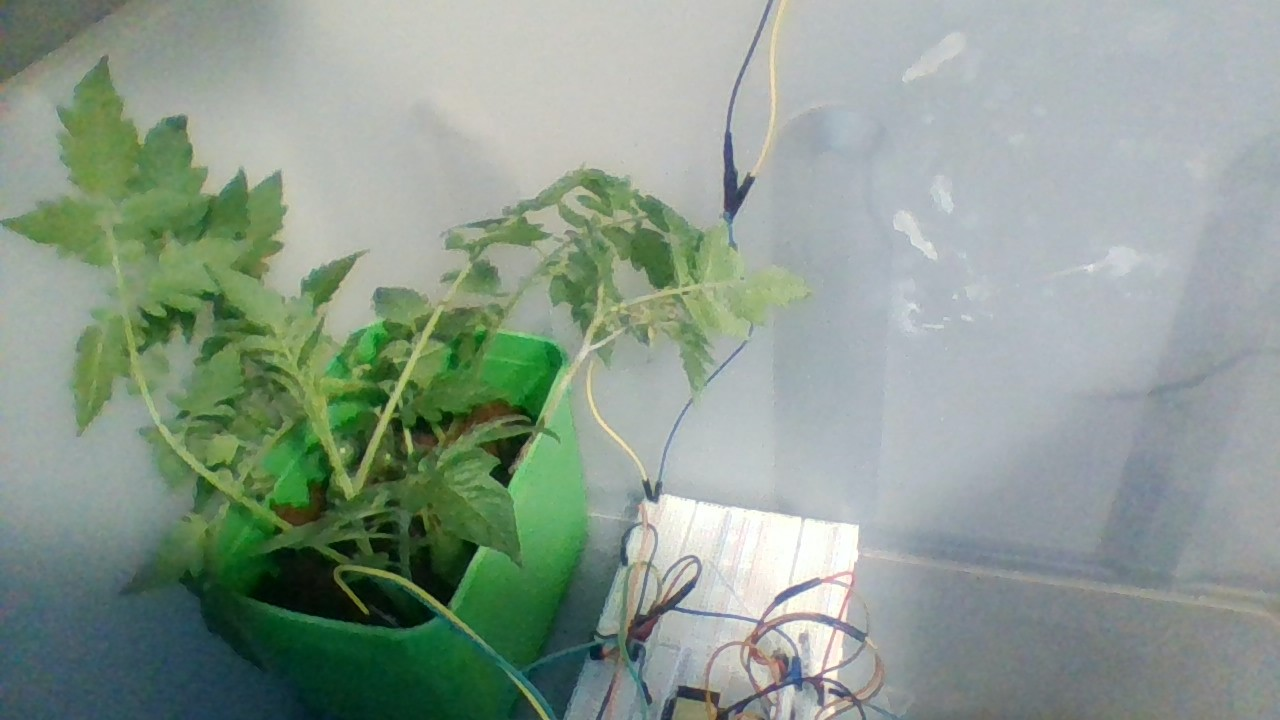
\includegraphics[width=.95\linewidth]{resultado1.jpg}\\[-2pt]
  {\small (a) Condição favorável}
\end{minipage}\hfill
\begin{minipage}{.46\textwidth}
  \centering
  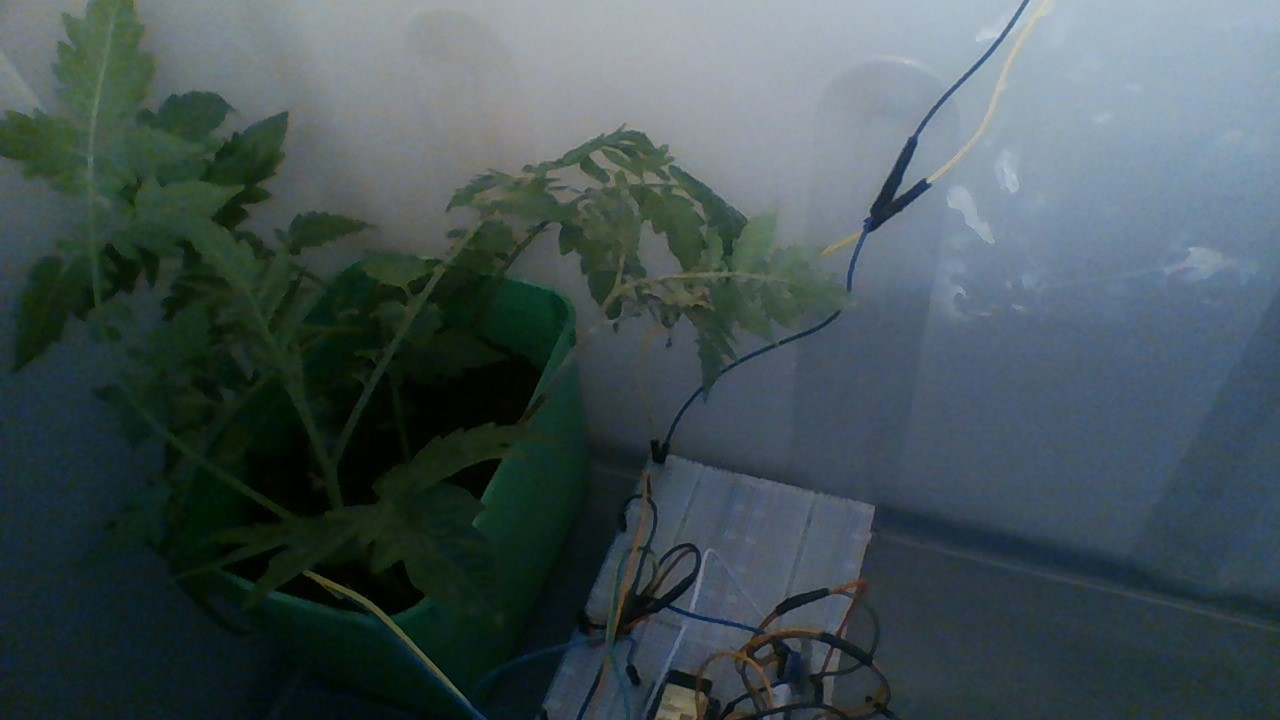
\includegraphics[width=.95\linewidth]{resultado3.jpg}\\[-2pt]
  {\small (b) Condição desfavorável}
\end{minipage}
\caption{Imagens reais capturadas em condições distintas de iluminação. Em (b),
a queda de brilho reduz a discriminabilidade dos descritores de cor,
aumentando a ambiguidade nas predições \textit{top-k}.}
\label{fig:res_real}
\end{figure}

\textit{Quality gates} baseados em cobertura de máscara segmentada e variância
do Laplaciano foram implementados para sinalizar imagens fora da distribuição
de treinamento. Como medidas de mitigação destacam-se: \textit{data augmentation}
fotométrico e reaquisição condicionada pelos \textit{quality gates}. Os
descritores de textura (Haralick, LBP) demonstraram maior estabilidade relativa
sob variações de brilho do que os histogramas de cor, sugerindo que pipelines
com maior peso em textura são inerentemente mais robustos a variações de
iluminação.

\FloatBarrier

\subsection{Comparação de Classificadores}

A Figura~\ref{fig:classifier_comparison} sintetiza os resultados dos três
classificadores clássicos e da baseline profunda.

\begin{figure}[ht]
\centering
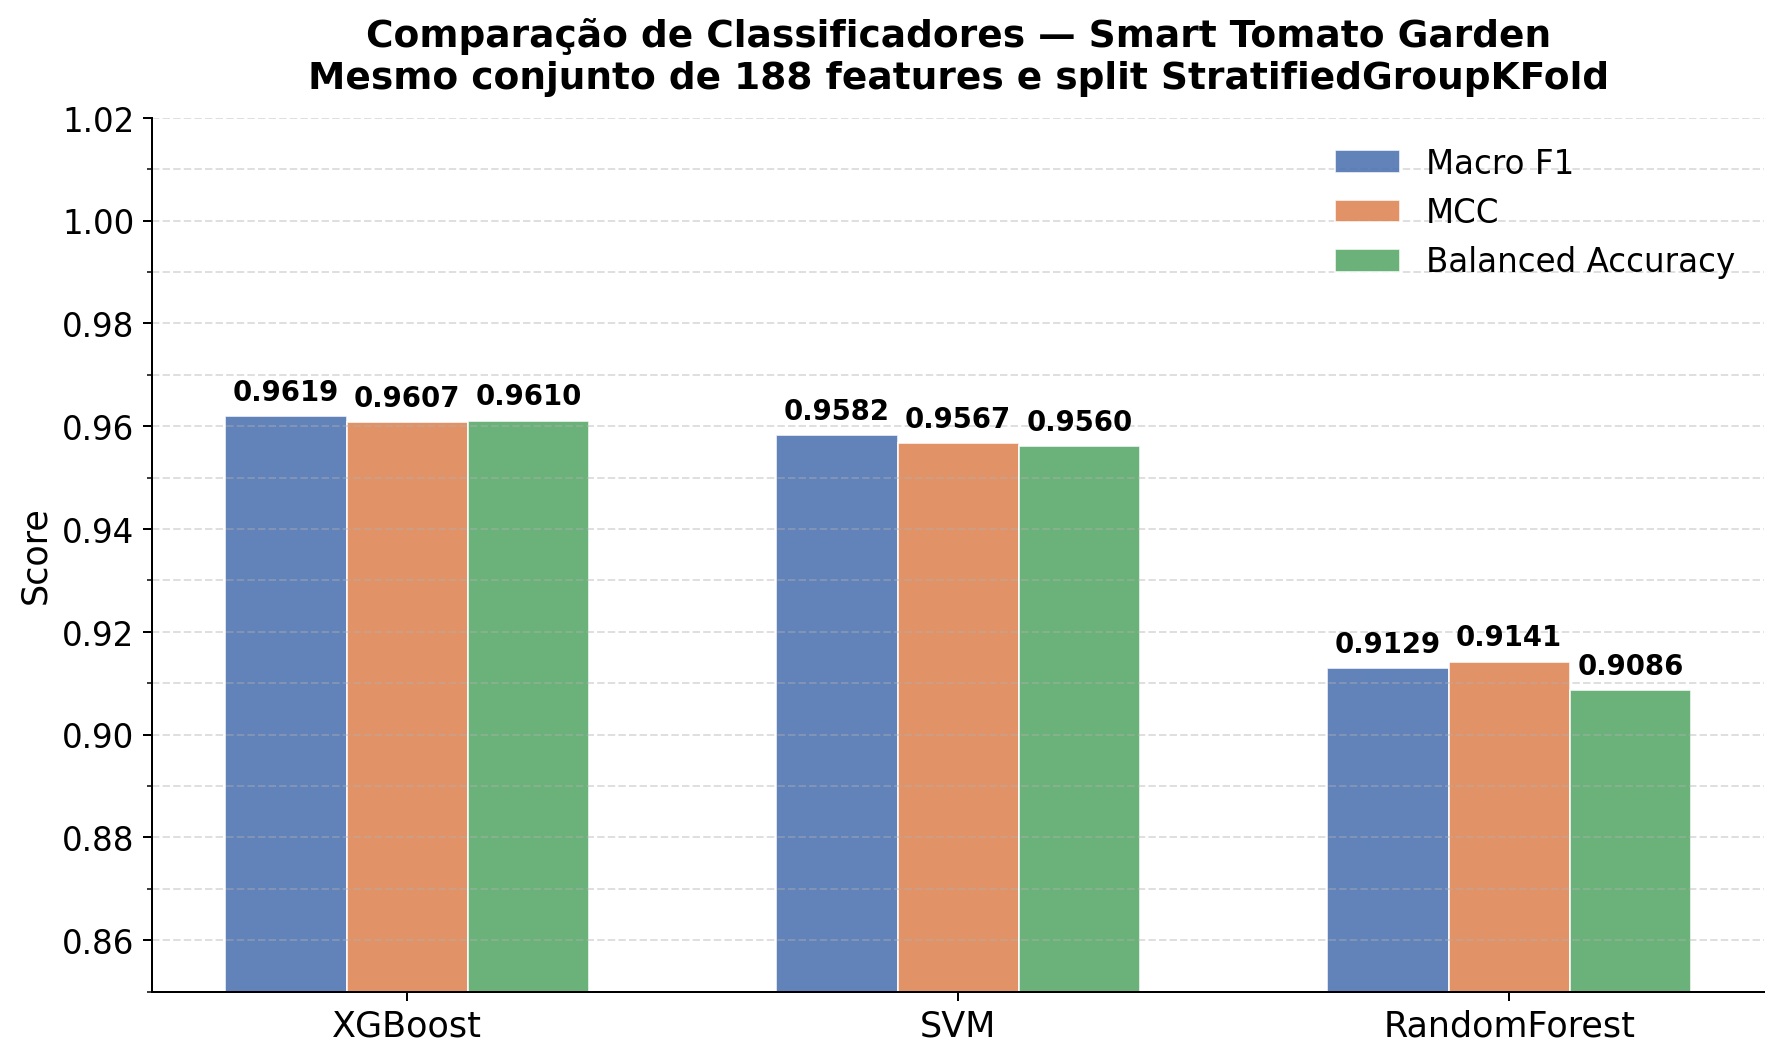
\includegraphics[width=.92\linewidth]{figuras/classifier_comparison.png}
\caption{Comparação entre \gls{XGBoost}, SVM e Random Forest em Macro~F1, MCC
e \textit{Balanced Accuracy}. Todos avaliados sobre os mesmos 188 atributos e
o mesmo conjunto de teste independente de 4.803 amostras.}
\label{fig:classifier_comparison}
\end{figure}

O \gls{XGBoost} (96,19\%, MCC 0,9607) superou o SVM em macro~F1
($+0{,}37$\,p.p.) e o Random Forest em $+4{,}9$\,p.p. A margem sobre o SVM é
pequena porém consistente: o SVM com kernel RBF ($C=10$, $\gamma=$\texttt{auto})
constitui alternativa viável quando a interpretabilidade de árvores não é
requisito. O Random Forest (91,29\%) oferece vantagem em velocidade de
treinamento ($\sim$6$\times$ mais rápido), sendo adequado para iterações
exploratórias e seleção de subconjuntos de atributos.

A MobileNetV3-Small (99,02\%) supera o \gls{XGBoost} em $+2{,}83$\,p.p. ao
aprender representações de ponta a ponta, mas com menor transparência interna.
O pipeline clássico tem como vantagem prática a interpretabilidade direta:
cada dimensão do vetor de atributos tem semântica conhecida, e a importância
de grupos de descritores pode ser analisada explicitamente.

\subsection{Importância de Atributos}

A análise de importância de atributos do \gls{XGBoost} --- calculada como
\textit{gain} médio por \textit{feature} sobre todas as árvores, agregada por
grupo --- revela que os descritores de textura concentram o maior poder
preditivo. O grupo Haralick/\gls{GLCM} e o LBP-NRI são os mais relevantes,
seguidos pelos histogramas \gls{HSV}. Descritores de forma (circularidade,
solidez, extensão) e cromaticidade contribuem marginalmente, indicando que a
discriminação entre classes de doença é primariamente textural e cromática,
não geométrica.

Esse padrão é coerente com a natureza das doenças: lesões como \textit{Early
Blight} e \textit{Target Spot} apresentam manchas concêntricas com gradiente
de cor e textura necrótica distintos da folha saudável, enquanto a geometria
da região afetada varia amplamente com o estágio da infecção. A baixa
contribuição dos atributos de forma sugere que investimento adicional em
descritores de textura de maior resolução (e.g., filtros de Gabor, LBP
multiescala) pode ser mais produtivo do que refinamento dos descritores
geométricos.

% NOTA: inserir figura de importância agregada por grupo após executar:
%   importances = pd.Series(model.feature_importances_, index=feature_names)
%   importances_by_group = importances.groupby(group_labels).sum().sort_values()
%   importances_by_group.plot(kind='barh')

\subsection{Análise por Classe}

A Tabela~\ref{tb:perclass} detalha o desempenho por classe do \gls{XGBoost}.

\begin{table}[ht]
\caption{F1-score por classe --- \gls{XGBoost} + 188 atributos (conjunto de
teste, 4.803 amostras)}
\label{tb:perclass}
\centering
\setlength{\tabcolsep}{5pt}
\renewcommand{\arraystretch}{1.1}
\begin{tabularx}{\textwidth}{Y c c c}
\toprule
\textbf{Classe} & \textbf{Precisão} & \textbf{Recall} & \textbf{F1} \\
\midrule
Bacterial Spot      & 97,51\% & 98,12\% & 97,81\% \\
Early Blight        & 94,55\% & 86,67\% & 90,43\% \\
Late Blight         & 95,28\% & 95,28\% & 95,28\% \\
Leaf Mold           & 96,82\% & 95,80\% & 96,31\% \\
Septoria Leaf Spot  & 95,91\% & 97,18\% & 96,54\% \\
Spider Mites        & 95,86\% & 96,62\% & 96,24\% \\
Target Spot         & 93,95\% & 95,96\% & 94,95\% \\
Yellow Leaf Curl    & 98,43\% & 97,82\% & 98,13\% \\
Mosaic Virus        & 97,35\% & 98,21\% & 97,78\% \\
Healthy             & 97,53\% & 99,37\% & 98,44\% \\
\bottomrule
\end{tabularx}
\end{table}

As maiores dificuldades concentram-se em \textit{Early Blight} (F1 90,43\%) e
\textit{Target Spot} (94,95\%), classes com lesões necrosantes de aparência
similar. Esse padrão de confusão é esperado para descritores de textura local
quando lesões estão em estágios iniciais ou sobrepostos. Classes com assinaturas
cromáticas distintas --- \textit{Yellow Leaf Curl} (98,13\%) e \textit{Healthy}
(98,44\%) --- obtiveram desempenho consistentemente elevado, corroborando a
dominância dos atributos de cor na separabilidade entre essas classes. A
confusão entre \textit{Early Blight} e \textit{Target Spot} sugere que
anotações por estágio de infecção ou por tipo de lesão poderiam melhorar o
treinamento nesses casos limítrofes.

\FloatBarrier

\subsection{Protocolo de Avaliação e Validade Estatística}

A avaliação de modelos em \textit{datasets} de doenças foliares enfrenta duas
ameaças comuns à validade interna: imagens da mesma folha ou planta
distribuídas entre treino e teste (\textit{data leakage} por grupo), e
duplicatas fotográficas que inflam o desempenho no conjunto de teste.

O protocolo adotado endereça ambas. O \textit{StratifiedGroupKFold} garante
que amostras do mesmo grupo de proveniência não coexistam em \textit{folds}
distintos durante a validação cruzada, preservando a estratificação de classes.
A deduplicação por \textit{SHA-256} remove cópias exatas antes da divisão,
eliminando uma fonte comum de otimismo nos resultados.

Para contextualizar o impacto: em \textit{splits} aleatórios sem controle de
grupo, classificadores clássicos treinados no PlantVillage tipicamente
reportam macro~F1 acima de 98\%~\cite{mohanty2016deep,zimmermann2025}. O
protocolo por grupos com deduplicação reduz essa estimativa para 96,19\%
no \gls{XGBoost}, 95,82\% no SVM e 91,29\% no Random Forest --- uma diferença
de $\sim$2--7 p.p.\ que indica vazamento nos protocolos de avaliação padrão.

Esse resultado tem implicação prática direta: sistemas avaliados com
\textit{splits} aleatórios no PlantVillage tendem a apresentar queda abrupta
de desempenho ao encontrar imagens de plantas fora do conjunto de treinamento
(i.e., nova safra, novo ambiente de captura). O protocolo por grupos produz
estimativas mais conservadoras e, portanto, mais confiáveis como preditor do
desempenho em campo.

\section{Conclusão}

Este trabalho apresentou um pipeline interpretável de \textit{feature engineering}
com 188 atributos organizados em 10 grupos para classificação de doenças
foliares em tomateiro, avaliado sob protocolo metodologicamente rigoroso com
\textit{StratifiedGroupKFold} e deduplicação \textit{SHA-256}. Entre os
classificadores clássicos, o \gls{XGBoost} obteve macro~F1 96,19\%
(MCC~0,9607), superando SVM ($+0{,}37$\,p.p.) e Random Forest ($+4{,}9$\,p.p.).
A MobileNetV3-Small atingiu 99,02\% como teto de desempenho com representações
aprendidas, com gap de $+2{,}83$\,p.p.\ sobre o melhor classificador clássico.

A análise de importância de atributos evidencia que textura (Haralick, LBP) e
cor (HSV) são os grupos primários de discriminação, enquanto forma contribui
marginalmente. O protocolo por grupos demonstra que \textit{splits} aleatórios
inflam as estimativas de desempenho em até $\sim$7\,p.p.\ em benchmarks como
o PlantVillage.

Como limitação, a validação depende integralmente do PlantVillage, conjunto
com características controladas. Como trabalhos futuros destacam-se:
(i)~validação com imagens \textit{in situ}; (ii)~seleção automática de
subgrupos de atributos para redução dimensional interpretável; e
(iii)~análise de confusão orientada a curadoria de dados para \textit{Early Blight}
e \textit{Target Spot}.

\bibliographystyle{sbc}
\bibliography{sbc-template}

\end{document}
